\subsection{User Registration And Setup Activity}

\begin{figure}[H]
    \centering
    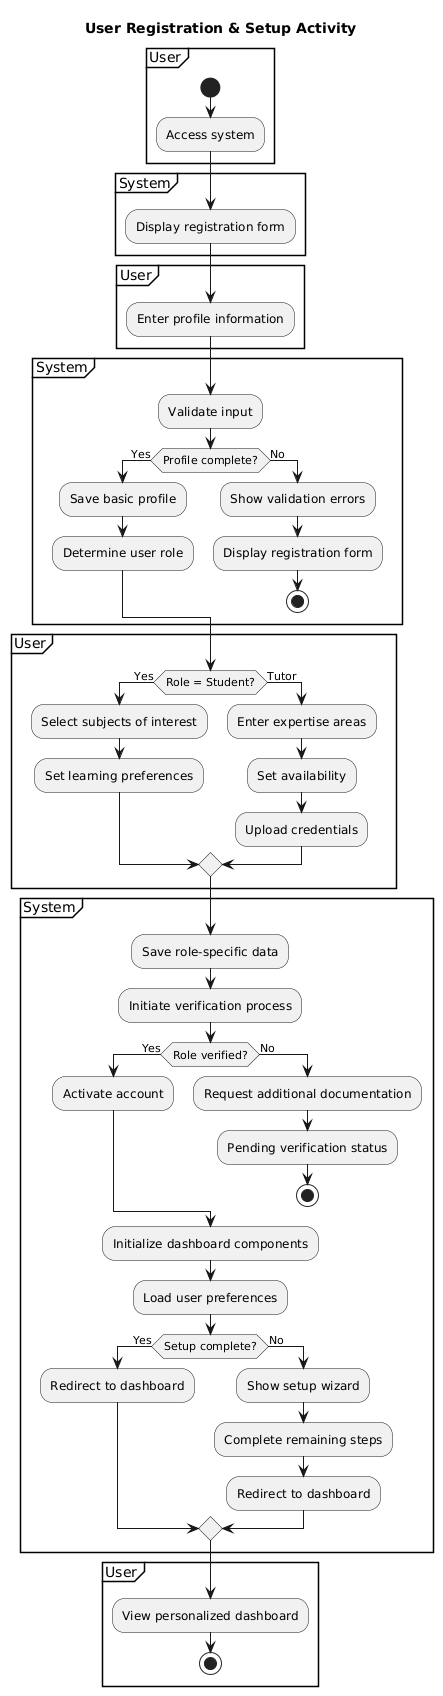
\includegraphics[width=0.3\textwidth]{graphics/chapter4/student/cc2.png}
    \caption{User Registration And Setup}
    \label{fig:Registration and Setup}
\end{figure}

\newpage 

\noindent \textbf{Description}
\begin{enumerate}
  \item \textbf{User}: Accesses system; initiates registration.
  \item \textbf{System}: Displays registration form.
  \item \textbf{User}: Enters profile information (name, email, ID, etc.).
  \item \textbf{System}: Validates input.
  \item \textbf{Decision}: Profile complete?
    \begin{enumerate}
        \item \textbf{Yes:} System saves basic profile; determines user role. Continue.
        \item \textbf{No:} System shows validation errors; displays registration form. \emph{Flow ends.}
    \end{enumerate}
  \item \textbf{User}: Performs role-specific setup based on assigned role.
    \begin{enumerate}
        \item \textbf{Student:} Selects subjects of interest; sets learning preferences.
        \item \textbf{Tutor:} Enters expertise areas; sets availability; uploads credentials.
    \end{enumerate}
  \item \textbf{System}: Saves role-specific data; initiates verification process.
  \item \textbf{Decision}: Role verified?
    \begin{enumerate}
        \item \textbf{Yes:} System activates account; grants role-based permissions. Continue.
        \item \textbf{No:} System requests additional documentation; sets pending verification status. \emph{Flow ends.}
    \end{enumerate}
  \item \textbf{System}: Initializes dashboard components; loads user preferences.
  \item \textbf{Decision}: Setup complete?
    \begin{enumerate}
        \item \textbf{Yes:} System redirects to role-specific dashboard. Continue.
        \item \textbf{No:} System shows setup wizard; completes remaining steps; redirects to dashboard.
    \end{enumerate}
  \item \textbf{User}: Views personalized dashboard. \textit{Flow ends.}
\end{enumerate}